% Options for packages loaded elsewhere
\PassOptionsToPackage{unicode}{hyperref}
\PassOptionsToPackage{hyphens}{url}
%
\documentclass[
]{book}
\usepackage{amsmath,amssymb}
\usepackage{lmodern}
\usepackage{iftex}
\ifPDFTeX
  \usepackage[T1]{fontenc}
  \usepackage[utf8]{inputenc}
  \usepackage{textcomp} % provide euro and other symbols
\else % if luatex or xetex
  \usepackage{unicode-math}
  \defaultfontfeatures{Scale=MatchLowercase}
  \defaultfontfeatures[\rmfamily]{Ligatures=TeX,Scale=1}
\fi
% Use upquote if available, for straight quotes in verbatim environments
\IfFileExists{upquote.sty}{\usepackage{upquote}}{}
\IfFileExists{microtype.sty}{% use microtype if available
  \usepackage[]{microtype}
  \UseMicrotypeSet[protrusion]{basicmath} % disable protrusion for tt fonts
}{}
\makeatletter
\@ifundefined{KOMAClassName}{% if non-KOMA class
  \IfFileExists{parskip.sty}{%
    \usepackage{parskip}
  }{% else
    \setlength{\parindent}{0pt}
    \setlength{\parskip}{6pt plus 2pt minus 1pt}}
}{% if KOMA class
  \KOMAoptions{parskip=half}}
\makeatother
\usepackage{xcolor}
\usepackage{longtable,booktabs,array}
\usepackage{calc} % for calculating minipage widths
% Correct order of tables after \paragraph or \subparagraph
\usepackage{etoolbox}
\makeatletter
\patchcmd\longtable{\par}{\if@noskipsec\mbox{}\fi\par}{}{}
\makeatother
% Allow footnotes in longtable head/foot
\IfFileExists{footnotehyper.sty}{\usepackage{footnotehyper}}{\usepackage{footnote}}
\makesavenoteenv{longtable}
\usepackage{graphicx}
\makeatletter
\def\maxwidth{\ifdim\Gin@nat@width>\linewidth\linewidth\else\Gin@nat@width\fi}
\def\maxheight{\ifdim\Gin@nat@height>\textheight\textheight\else\Gin@nat@height\fi}
\makeatother
% Scale images if necessary, so that they will not overflow the page
% margins by default, and it is still possible to overwrite the defaults
% using explicit options in \includegraphics[width, height, ...]{}
\setkeys{Gin}{width=\maxwidth,height=\maxheight,keepaspectratio}
% Set default figure placement to htbp
\makeatletter
\def\fps@figure{htbp}
\makeatother
\setlength{\emergencystretch}{3em} % prevent overfull lines
\providecommand{\tightlist}{%
  \setlength{\itemsep}{0pt}\setlength{\parskip}{0pt}}
\setcounter{secnumdepth}{5}
\usepackage{booktabs}
\usepackage{booktabs}
\usepackage{longtable}
\usepackage{array}
\usepackage{multirow}
\usepackage{wrapfig}
\usepackage{float}
\usepackage{colortbl}
\usepackage{pdflscape}
\usepackage{tabu}
\usepackage{threeparttable}
\usepackage{threeparttablex}
\usepackage[normalem]{ulem}
\usepackage{makecell}
\usepackage{xcolor}
\usepackage{fontspec}
\usepackage{multicol}
\usepackage{hhline}
\usepackage{hyperref}
\usepackage{hhline}
\newlength\Oldarrayrulewidth
\newlength\Oldtabcolsep
\ifLuaTeX
  \usepackage{selnolig}  % disable illegal ligatures
\fi
\usepackage[]{natbib}
\bibliographystyle{plainnat}
\IfFileExists{bookmark.sty}{\usepackage{bookmark}}{\usepackage{hyperref}}
\IfFileExists{xurl.sty}{\usepackage{xurl}}{} % add URL line breaks if available
\urlstyle{same} % disable monospaced font for URLs
\hypersetup{
  pdftitle={Greenhouse Gas Emissions Scenario Planning},
  pdfauthor={Metropolitan Council},
  hidelinks,
  pdfcreator={LaTeX via pandoc}}

\title{Greenhouse Gas Emissions Scenario Planning}
\author{Metropolitan Council}
\date{January 2023}

\begin{document}
\maketitle

{
\setcounter{tocdepth}{1}
\tableofcontents
}
\hypertarget{greenhouse-gas-scenario-planning}{%
\chapter*{Greenhouse Gas Scenario Planning}\label{greenhouse-gas-scenario-planning}}
\addcontentsline{toc}{chapter}{Greenhouse Gas Scenario Planning}

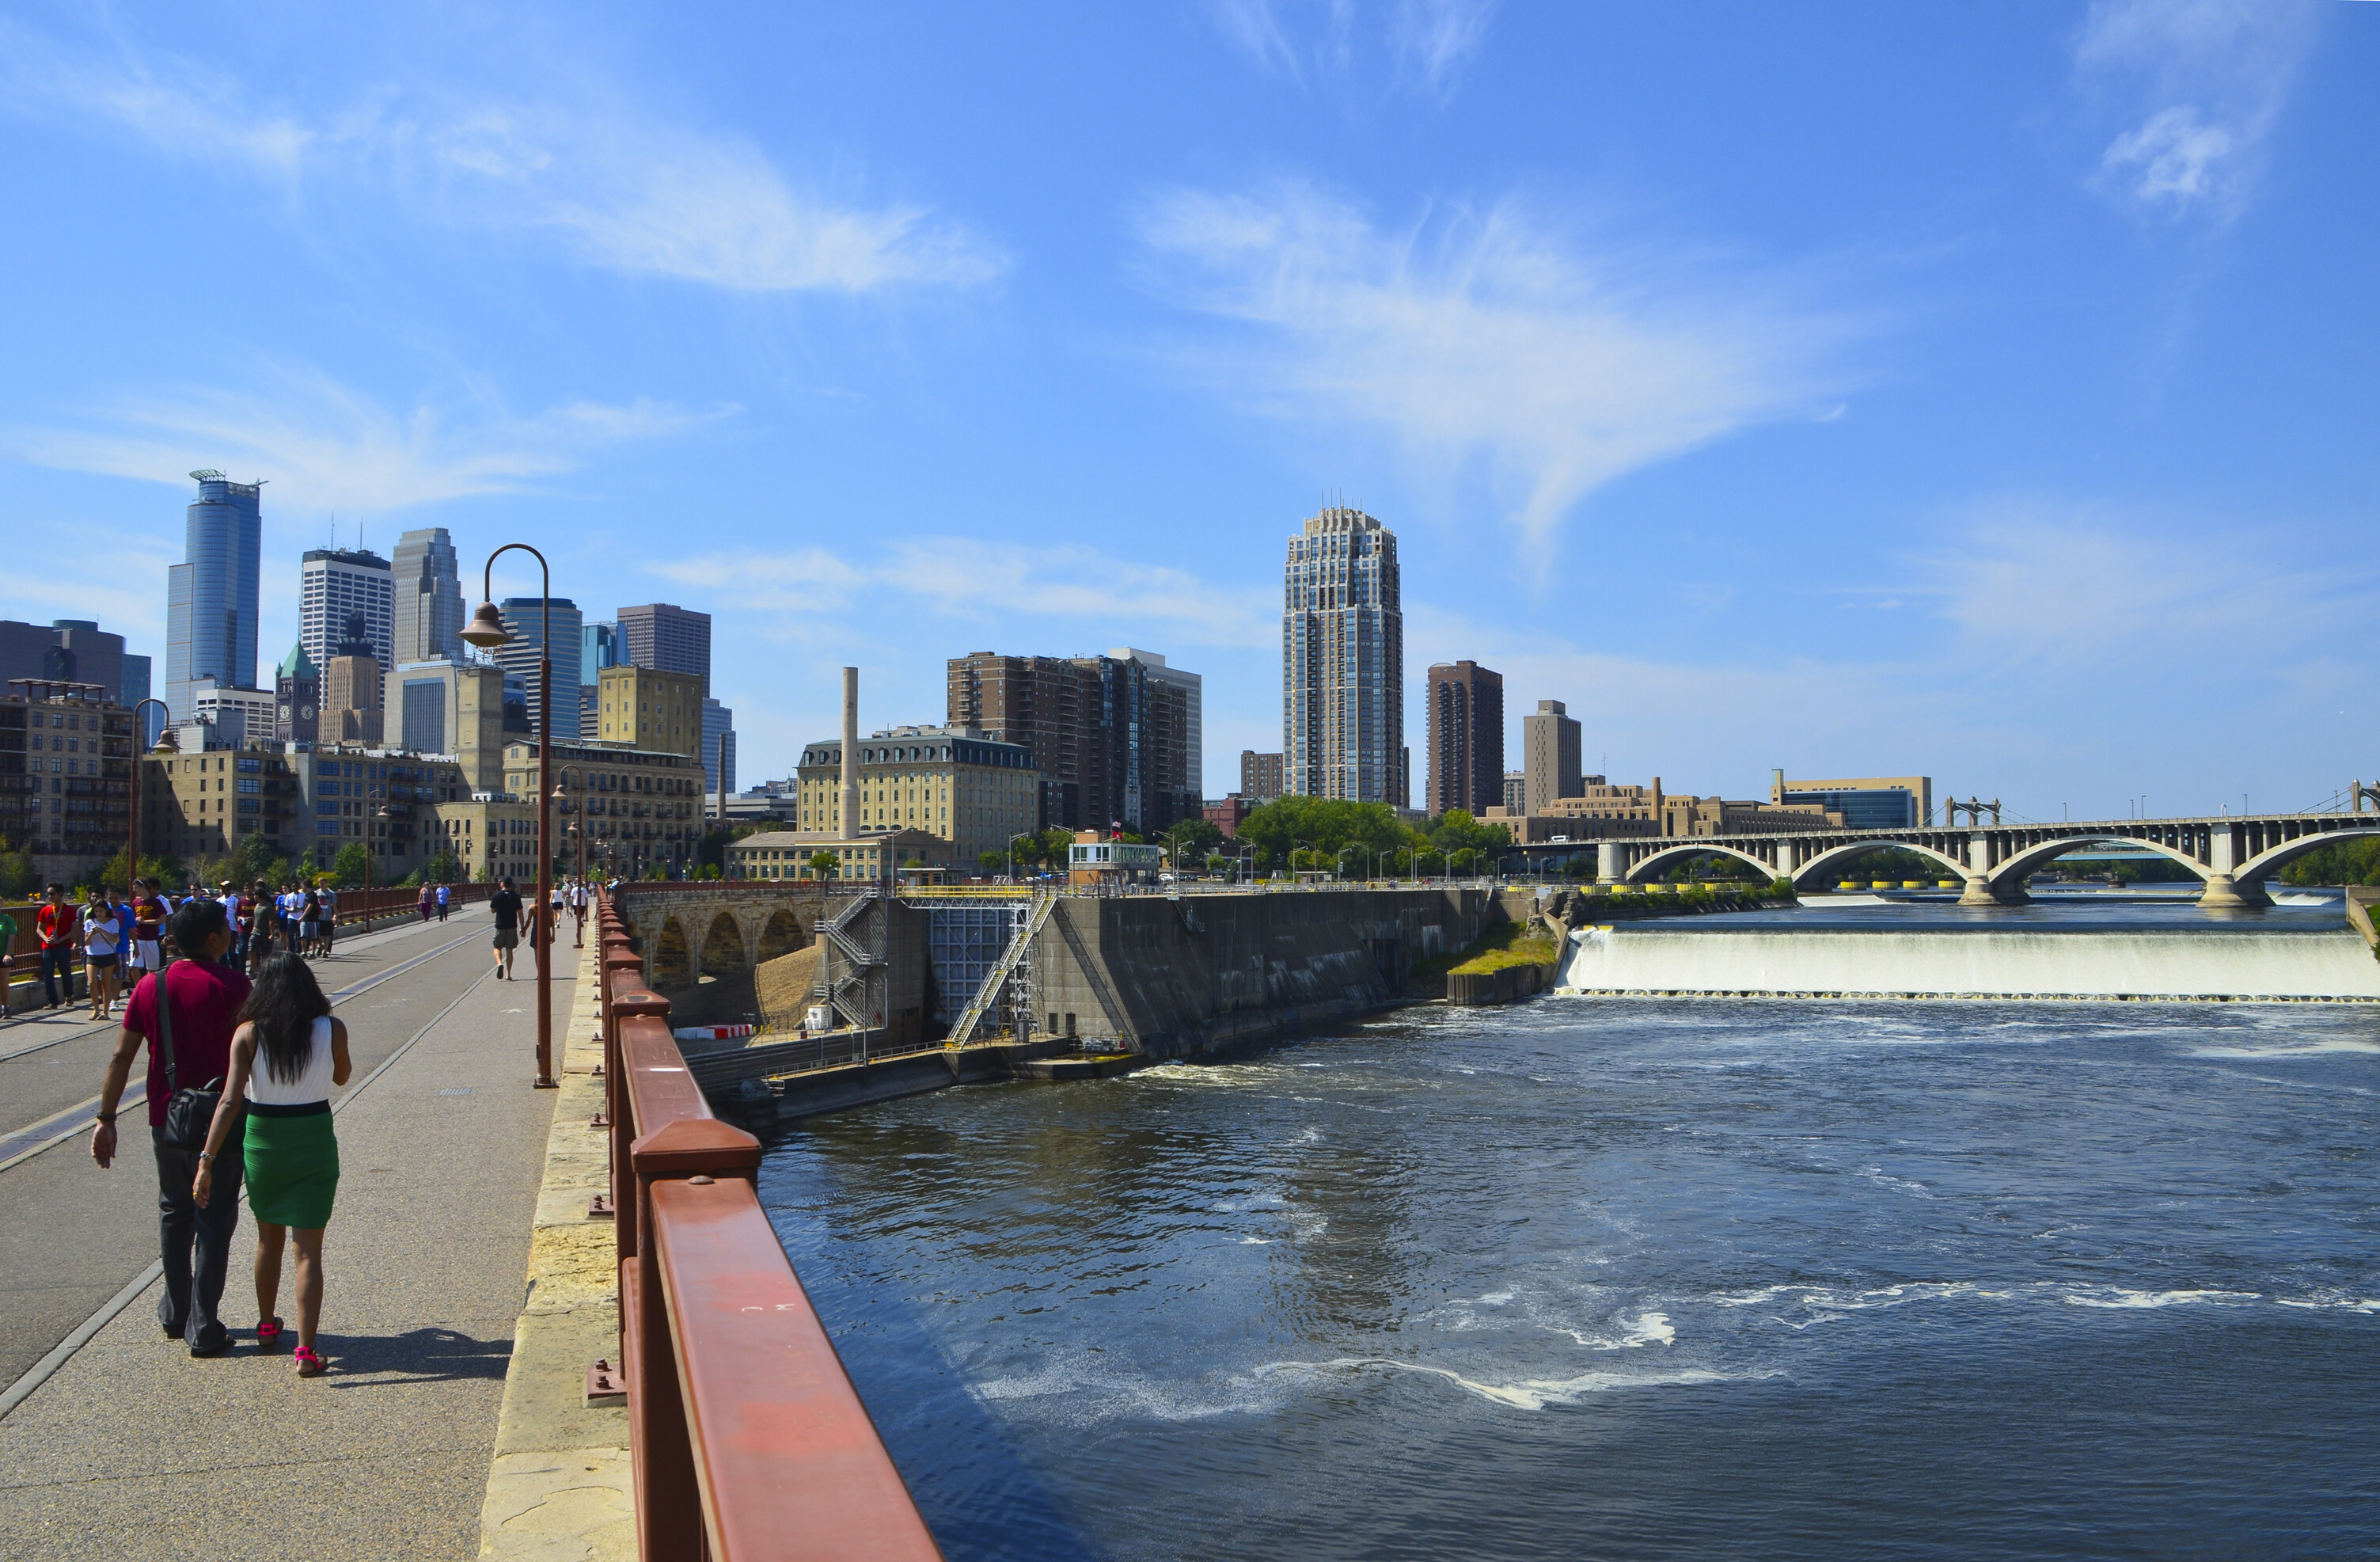
\includegraphics{images/2788.jpg}

\hypertarget{metropolitan-council}{%
\section*{Metropolitan Council}\label{metropolitan-council}}
\addcontentsline{toc}{section}{Metropolitan Council}

\global\setlength{\Oldarrayrulewidth}{\arrayrulewidth}

\global\setlength{\Oldtabcolsep}{\tabcolsep}

\setlength{\tabcolsep}{0pt}

\renewcommand*{\arraystretch}{1.5}



\providecommand{\ascline}[3]{\noalign{\global\arrayrulewidth #1}\arrayrulecolor[HTML]{#2}\cline{#3}}

\begin{longtable}[c]{|p{1.93in}|p{0.98in}|p{1.90in}|p{1.08in}}





\multicolumn{1}{>{\raggedright}p{\dimexpr 1.93in+0\tabcolsep}}{\textcolor[HTML]{000000}{\fontsize{11}{11}\selectfont{\global\setmainfont{DejaVu Sans}{Charlie\ Zelle}}}} & \multicolumn{1}{>{\raggedright}p{\dimexpr 0.98in+0\tabcolsep}}{\textcolor[HTML]{000000}{\fontsize{11}{11}\selectfont{\global\setmainfont{DejaVu Sans}{Chair}}}} & \multicolumn{1}{>{\raggedright}p{\dimexpr 1.9in+0\tabcolsep}}{\textcolor[HTML]{000000}{\fontsize{11}{11}\selectfont{\global\setmainfont{DejaVu Sans}{Raymond\ Zeran}}}} & \multicolumn{1}{>{\raggedright}p{\dimexpr 1.08in+0\tabcolsep}}{\textcolor[HTML]{000000}{\fontsize{11}{11}\selectfont{\global\setmainfont{DejaVu Sans}{District\ 9}}}} \\





\multicolumn{1}{>{\raggedright}p{\dimexpr 1.93in+0\tabcolsep}}{\textcolor[HTML]{000000}{\fontsize{11}{11}\selectfont{\global\setmainfont{DejaVu Sans}{Judy\ Johnson}}}} & \multicolumn{1}{>{\raggedright}p{\dimexpr 0.98in+0\tabcolsep}}{\textcolor[HTML]{000000}{\fontsize{11}{11}\selectfont{\global\setmainfont{DejaVu Sans}{District\ 1}}}} & \multicolumn{1}{>{\raggedright}p{\dimexpr 1.9in+0\tabcolsep}}{\textcolor[HTML]{000000}{\fontsize{11}{11}\selectfont{\global\setmainfont{DejaVu Sans}{Peter\ Lindstrom}}}} & \multicolumn{1}{>{\raggedright}p{\dimexpr 1.08in+0\tabcolsep}}{\textcolor[HTML]{000000}{\fontsize{11}{11}\selectfont{\global\setmainfont{DejaVu Sans}{District\ 10}}}} \\





\multicolumn{1}{>{\raggedright}p{\dimexpr 1.93in+0\tabcolsep}}{\textcolor[HTML]{000000}{\fontsize{11}{11}\selectfont{\global\setmainfont{DejaVu Sans}{Reva\ Chamblis}}}} & \multicolumn{1}{>{\raggedright}p{\dimexpr 0.98in+0\tabcolsep}}{\textcolor[HTML]{000000}{\fontsize{11}{11}\selectfont{\global\setmainfont{DejaVu Sans}{District\ 2}}}} & \multicolumn{1}{>{\raggedright}p{\dimexpr 1.9in+0\tabcolsep}}{\textcolor[HTML]{000000}{\fontsize{11}{11}\selectfont{\global\setmainfont{DejaVu Sans}{Susan\ Vento}}}} & \multicolumn{1}{>{\raggedright}p{\dimexpr 1.08in+0\tabcolsep}}{\textcolor[HTML]{000000}{\fontsize{11}{11}\selectfont{\global\setmainfont{DejaVu Sans}{District\ 11}}}} \\





\multicolumn{1}{>{\raggedright}p{\dimexpr 1.93in+0\tabcolsep}}{\textcolor[HTML]{000000}{\fontsize{11}{11}\selectfont{\global\setmainfont{DejaVu Sans}{Christopher\ Ferguson}}}} & \multicolumn{1}{>{\raggedright}p{\dimexpr 0.98in+0\tabcolsep}}{\textcolor[HTML]{000000}{\fontsize{11}{11}\selectfont{\global\setmainfont{DejaVu Sans}{District\ 3}}}} & \multicolumn{1}{>{\raggedright}p{\dimexpr 1.9in+0\tabcolsep}}{\textcolor[HTML]{000000}{\fontsize{11}{11}\selectfont{\global\setmainfont{DejaVu Sans}{Francisco\ J.\ Gonzalez}}}} & \multicolumn{1}{>{\raggedright}p{\dimexpr 1.08in+0\tabcolsep}}{\textcolor[HTML]{000000}{\fontsize{11}{11}\selectfont{\global\setmainfont{DejaVu Sans}{District\ 12}}}} \\





\multicolumn{1}{>{\raggedright}p{\dimexpr 1.93in+0\tabcolsep}}{\textcolor[HTML]{000000}{\fontsize{11}{11}\selectfont{\global\setmainfont{DejaVu Sans}{Deb\ Barber}}}} & \multicolumn{1}{>{\raggedright}p{\dimexpr 0.98in+0\tabcolsep}}{\textcolor[HTML]{000000}{\fontsize{11}{11}\selectfont{\global\setmainfont{DejaVu Sans}{District\ 4}}}} & \multicolumn{1}{>{\raggedright}p{\dimexpr 1.9in+0\tabcolsep}}{\textcolor[HTML]{000000}{\fontsize{11}{11}\selectfont{\global\setmainfont{DejaVu Sans}{Chai\ Lee}}}} & \multicolumn{1}{>{\raggedright}p{\dimexpr 1.08in+0\tabcolsep}}{\textcolor[HTML]{000000}{\fontsize{11}{11}\selectfont{\global\setmainfont{DejaVu Sans}{District\ 13}}}} \\





\multicolumn{1}{>{\raggedright}p{\dimexpr 1.93in+0\tabcolsep}}{\textcolor[HTML]{000000}{\fontsize{11}{11}\selectfont{\global\setmainfont{DejaVu Sans}{Molly\ Cummings}}}} & \multicolumn{1}{>{\raggedright}p{\dimexpr 0.98in+0\tabcolsep}}{\textcolor[HTML]{000000}{\fontsize{11}{11}\selectfont{\global\setmainfont{DejaVu Sans}{District\ 5}}}} & \multicolumn{1}{>{\raggedright}p{\dimexpr 1.9in+0\tabcolsep}}{\textcolor[HTML]{000000}{\fontsize{11}{11}\selectfont{\global\setmainfont{DejaVu Sans}{Kris\ Fredson}}}} & \multicolumn{1}{>{\raggedright}p{\dimexpr 1.08in+0\tabcolsep}}{\textcolor[HTML]{000000}{\fontsize{11}{11}\selectfont{\global\setmainfont{DejaVu Sans}{District\ 14}}}} \\





\multicolumn{1}{>{\raggedright}p{\dimexpr 1.93in+0\tabcolsep}}{\textcolor[HTML]{000000}{\fontsize{11}{11}\selectfont{\global\setmainfont{DejaVu Sans}{John\ Pacheco\ Jr.}}}} & \multicolumn{1}{>{\raggedright}p{\dimexpr 0.98in+0\tabcolsep}}{\textcolor[HTML]{000000}{\fontsize{11}{11}\selectfont{\global\setmainfont{DejaVu Sans}{District\ 6}}}} & \multicolumn{1}{>{\raggedright}p{\dimexpr 1.9in+0\tabcolsep}}{\textcolor[HTML]{000000}{\fontsize{11}{11}\selectfont{\global\setmainfont{DejaVu Sans}{Phillip\ Sterner}}}} & \multicolumn{1}{>{\raggedright}p{\dimexpr 1.08in+0\tabcolsep}}{\textcolor[HTML]{000000}{\fontsize{11}{11}\selectfont{\global\setmainfont{DejaVu Sans}{District\ 15}}}} \\





\multicolumn{1}{>{\raggedright}p{\dimexpr 1.93in+0\tabcolsep}}{\textcolor[HTML]{000000}{\fontsize{11}{11}\selectfont{\global\setmainfont{DejaVu Sans}{Robert\ Lilligren}}}} & \multicolumn{1}{>{\raggedright}p{\dimexpr 0.98in+0\tabcolsep}}{\textcolor[HTML]{000000}{\fontsize{11}{11}\selectfont{\global\setmainfont{DejaVu Sans}{District\ 7}}}} & \multicolumn{1}{>{\raggedright}p{\dimexpr 1.9in+0\tabcolsep}}{\textcolor[HTML]{000000}{\fontsize{11}{11}\selectfont{\global\setmainfont{DejaVu Sans}{Wendy\ Wulff}}}} & \multicolumn{1}{>{\raggedright}p{\dimexpr 1.08in+0\tabcolsep}}{\textcolor[HTML]{000000}{\fontsize{11}{11}\selectfont{\global\setmainfont{DejaVu Sans}{District\ 16}}}} \\





\multicolumn{1}{>{\raggedright}p{\dimexpr 1.93in+0\tabcolsep}}{\textcolor[HTML]{000000}{\fontsize{11}{11}\selectfont{\global\setmainfont{DejaVu Sans}{Abdirahman\ Muse}}}} & \multicolumn{1}{>{\raggedright}p{\dimexpr 0.98in+0\tabcolsep}}{\textcolor[HTML]{000000}{\fontsize{11}{11}\selectfont{\global\setmainfont{DejaVu Sans}{District\ 8}}}} & \multicolumn{1}{>{\raggedright}p{\dimexpr 1.9in+0\tabcolsep}}{\textcolor[HTML]{000000}{\fontsize{11}{11}\selectfont{\global\setmainfont{DejaVu Sans}{}}}} & \multicolumn{1}{>{\raggedright}p{\dimexpr 1.08in+0\tabcolsep}}{\textcolor[HTML]{000000}{\fontsize{11}{11}\selectfont{\global\setmainfont{DejaVu Sans}{}}}} \\

\ascline{2pt}{666666}{1-4}



\end{longtable}



\arrayrulecolor[HTML]{000000}

\global\setlength{\arrayrulewidth}{\Oldarrayrulewidth}

\global\setlength{\tabcolsep}{\Oldtabcolsep}

\renewcommand*{\arraystretch}{1}

\leavevmode\vadjust pre{\hypertarget{top_container}{}}%
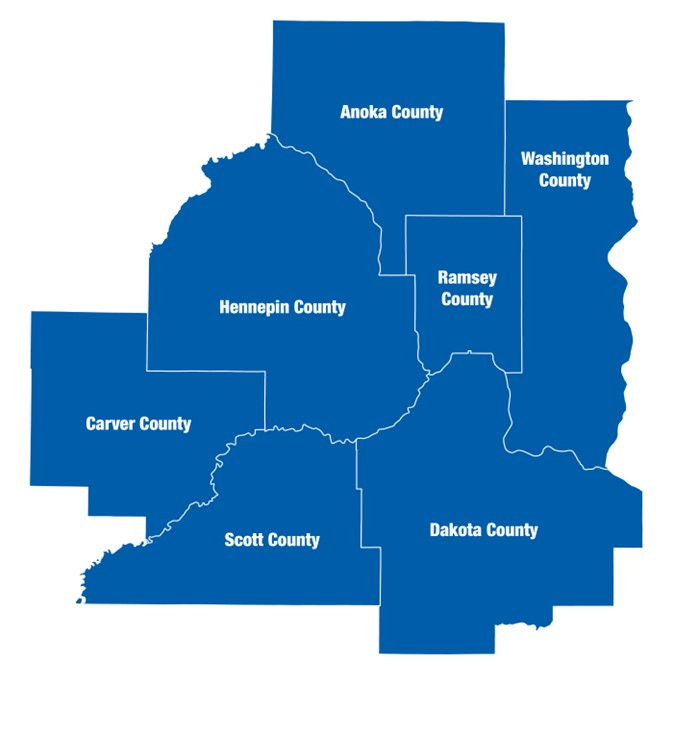
\includegraphics[width=0.85\textwidth,height=\textheight]{images/map.jpg}

\leavevmode\vadjust pre{\hypertarget{top_right}{}}%
The Metropolitan Council is the regional planning organization for the seven-county Twin Cities area. The Council operates the regional bus and rail system, collects and treats wastewater, coordinates regional water resources, plans and helps fund regional parks, and administers federal funds that provide housing opportunities for low- and moderate-income individuals and families. The 17-member Council board is appointed by and serves at the pleasure of the governor.

On request, this publication will be made available in alternative formats to people with disabilities. Call Metropolitan Council information at 651-602-1140 or TTY 651-291-0904

\hypertarget{disclaimer}{%
\section*{Disclaimer}\label{disclaimer}}
\addcontentsline{toc}{section}{Disclaimer}

This report aims to evaluate the effectiveness of greenhouse gas (GHG) mitigation strategies at the city level. It is intended to provide information that can be used to support policy discussions and educational purposes. Please note that the report is for informational purposes only and does not constitute official recommendations or policy decisions.

\hypertarget{executive-summary}{%
\section*{Executive Summary}\label{executive-summary}}
\addcontentsline{toc}{section}{Executive Summary}

The Research Unit of Community Development at the Metropolitan Council has prepared the following report, which presents a range of strategies that the City of Minneapolis could adopt to reduce greenhouse gas emissions relative to a ``Business as Usual'' scenario. These strategies are divided into three categories: stationary energy (building sector), transportation, and land use and forestry. It is worth noting that the greenhouse gas emissions estimates presented in this report may differ from those found in the Minneapolis Greenhouse Gas Inventory due to differences in methodology. The strategies included in this report were decided in a series of stakeholder meetings conducted in 2020.

\hypertarget{introduction}{%
\chapter{Introduction}\label{introduction}}

\hypertarget{overview}{%
\section{Overview}\label{overview}}

Cities throughout the Minnesota Metro Region are well aware of the pressing need to reduce greenhouse gas emissions and enhance the resilience of their communities in the face of climate change. In recognition of this urgency, many of these cities, including Minneapolis, have already begun implementing various strategies and initiatives to reduce their carbon footprint and increase their ability to withstand the impacts of a changing climate. These efforts range from adopting renewable energy sources and energy-efficient technologies to implementing transportation policies that encourage using electric or low-emissions vehicles to promote land use practices that support the retention and expansion of natural habitats. By taking action at the local level, local governments in the Twin Cities contribute to the global effort to mitigate the worst effects of climate change and build a more sustainable and equitable future.

This report aims to support the City of Minneapolis in considering potential strategies for reducing carbon emissions. The Metropolitan Council seeks to expand the information and technical assistance it provides to local governments to support regional and local climate change planning. The Council offers tools and guidance to help get cities on track to meet local, regional, and state goals.

\hypertarget{greenhouse-gas-emissions}{%
\section{Greenhouse Gas Emissions}\label{greenhouse-gas-emissions}}

Greenhouse gases (GHG) trap heat in the atmosphere and contribute to global warming. Carbon dioxide, methane, and nitrous oxide are the most common greenhouse gases. Human activities have been the primary driver of climate change by releasing greenhouse gases in large amounts. Combustion of fossil fuels (e.g., coal, oil, and natural gas) releases greenhouse gases, which trap heat in the atmosphere, causing temperatures to rise.

The primary sources of emissions in cities come from building energy use (electricity and natural gas), transportation (gas and diesel), and waste (methane at landfills or combustion for energy generation). The transportation sector, which includes cars, trucks, ships, and airplanes, is the largest source of carbon dioxide emissions in the United States, followed by the electricity and heat production and industrial sectors. Other sources of greenhouse gas emissions in Minnesota include agriculture, waste, and industrial processes.

\hypertarget{impact-of-climate-change-in-minnesota}{%
\section{Impact of Climate Change in Minnesota}\label{impact-of-climate-change-in-minnesota}}

The climate in Minnesota is changing, leading to more extreme rain events, heat waves, and drought. These changes will have significant impacts on transportation, waste water services, and water resources in the region.

Extreme heat events will increase water demand, leading to higher energy use, treatment costs, and lower efficiency in water supply systems. More extreme rain events will lead to more erosion, rainwater runoff, and flooding, disrupting transportation operations and damaging sewer and storm-water systems. Drought will lead to lower groundwater levels, stressed water resources, and more algal blooms and fish kills. These impacts will disproportionately affect marginalized communities and require the region to adapt and become more resilient to these changes.

\hypertarget{scenario-planning}{%
\section{Scenario Planning}\label{scenario-planning}}

The Metropolitan Council has developed a Greenhouse Gas Scenario Planning Tool to help metro cities determine pathways to achieving emissions reductions. The Tool builds upon the DECAL model created by the Sustainable Healthy Cities Network with the support and funding of the Metropolitan Council.

Scenario planning is a method to make flexible long-term plans. It is a way of thinking about and preparing for the future by considering possible events and their potential impact on a city or region. Scenario planning involves creating multiple possible future scenarios and then considering how to respond to each one. This method allows organizations to be more flexible and adaptable in uncertainty and change.

The Greenhouse Gas Scenario Planning Tool looks at strategies across multiple sectors and calculates the emissions reductions that can result from successful implementation. These sectors include compact land use, mobility, buildings, waste, and green infrastructure.

The Metropolitan Council will offer the scenario planning tool on an easy-to-use online platform. Cities can use this Tool to identify solutions tailored to their communities by testing different scenarios across strategies.

The following report compiles the City of Minneapolis results based on the Greenhouse Gas Scenario Planning Tool created by the Metropolitan Council and adapted from the collaborative work between the Sustainable Healthy Cities Network and the Metropolitan Council.

\hypertarget{stakeholder-engagement}{%
\section{Stakeholder Engagement}\label{stakeholder-engagement}}

In April and May of 2022, the Metropolitan Council conducted a series of community stakeholder engagement sessions to gather input regarding crucial considerations in designing the Greenhouse Gas Scenario Planning Tool. The stakeholder meetings were organized by different interest groups, which included local governments and counties, non-profit think tanks, advocacy groups, private consulting firms, academia, and staff from different divisions at the Metropolitan Council.

The stakeholders identified several priorities for developing the Greenhouse Gas Scenario Planning Tool, including (in ranking order) vehicle electrification, grid renewables, building retrofits, mixed-use development, and building codes.

\hypertarget{vehicle-electrification}{%
\subsection{Vehicle Electrification}\label{vehicle-electrification}}

Vehicle electrification ranked first in a list of strategies stakeholders wanted to explore in the Greenhouse Gas Scenario Planning Tool because it has the potential to reduce greenhouse gas emissions and improve air quality in the transportation sector. During the stakeholder engagement, the community members emphasized the trend towards electrification of short trips in the vehicle industry and the need to factor in changes to the grid electricity mix as electric vehicle adoption increases. They also emphasized the importance of quickly adopting electric vehicles and reducing vehicle miles traveled (VMT) to achieve environmental justice and improve air quality. The stakeholders asked if it is possible to model the effects of EV adoption on localized pollution. Overall, the community members emphasized the potential benefits of vehicle electrification and the need to consider its impacts on the grid and local air quality.

\hypertarget{grid-renewables}{%
\subsection{Grid Renewables}\label{grid-renewables}}

``Grid renewables'' refer to using renewable energy sources, such as solar or wind power, to generate electricity for the grid. During the stakeholder engagement sessions, community members highlighted the importance of modeling grid renewables because it is a significant emission lever, even though it is not within local government control and is often already modeled by utilities. Local governments can influence the grid mix by working together and speaking with a unified voice. They can also purchase \href{https://www.leg.mn.gov/docs/2019/mandated/190330.pdf}{Renewable Energy Certificates}\footnote{The Minnesota Statute section 216B.1691 was amended in 2003 and 2007 to allow for the establishment of a program for tradable Renewable Energy Credits (RECs). The Public Utilities Commission was required to establish this program by 2008 and to require all electric utilities to participate in a Commission-approved REC tracking system. In 2007, the Commission approved the use of the \href{https://www.mrets.org/}{Midwest Renewable Energy Tracking System} (M-RETS) as the REC tracking system and set a four-year shelf life for RECs. This means that RECs are eligible to be used to meet Renewable Energy Standard (RES) requirements in the year they are generated and for four years afterwards. In 2008, the Commission directed utilities to retire RECs equivalent to 1\% of their Minnesota annual retail sales by May 1st of the following year. These retired RECs are transferred to a specific Minnesota RES retirement account and cannot be used to meet other state or program requirements. Utilities must submit an annual compliance filing demonstrating their compliance with the RES by June 1st.} (RECs) to obtain green power. The ownership of solar assets and the retirement of RECs can affect the benefits and amount of renewable energy added to the grid through community solar projects. Focusing on grid renewables and community solar can maximize equity benefits and is more important than improving access to rooftop solar.

\hypertarget{building-retrofits}{%
\subsection{Building Retrofits}\label{building-retrofits}}

During the stakeholder engagement, the community members commented that building retrofits are vital because they can increase energy efficiency, which could benefit low-income people the most. It is important to model more high-level, general strategies that will be relevant in the future rather than more specific, short-term strategies that may be affected by changing circumstances or policy priorities. Building retrofits have the potential for city and utility collaboration, as utilities often offer tools and programs to increase efficiency. The feasibility and cost of building electrification should be considered to ensure that it benefits the community beyond reducing emissions. It may also be beneficial to consider participation in the new ``\emph{LEED for Communities}'' program. Commercial building energy benchmarking may be more effective than focusing on residential buildings.

\hypertarget{mixed-use-development}{%
\subsection{Mixed-Use Development}\label{mixed-use-development}}

Mixed-use development involves building buildings with multiple functions, such as housing, offices, and retail spaces, in a single location. Unlike many other strategies, such as increasing grid renewables or improving building codes, which may be outside local government control, the stakeholder mentioned that mixed-use development is within the control of local governments. Local governments have the authority to regulate land use and development in their jurisdictions, including the construction of mixed-use buildings.

\hypertarget{building-codes}{%
\subsection{Building Codes}\label{building-codes}}

Building codes refer to the regulations and standards governing building design and construction, including energy efficiency requirements. These priorities can help to create more sustainable and livable communities. The report discusses the impact of building standards such as LEED Gold for residential development.

  \bibliography{book.bib,packages.bib}

\end{document}
